\newpage
\section{Introdução}

\section{Erro na tensão de saída}
Apesar das equações desenvolvidas na teoria, os circuitos conversores de potência geralmente não apresentam, de forma precisa, a mesma tensão de saída que a calculada. Isso se deve ao fato da variação da tensão de entrada, na variação nos parâmetros dos componentes, das componentes parasitas, as perdas no circuito e variações no ambiente, como a variação da temperatura.
Esse erro na tensão de saída pode tornar inviável o uso de um conversor em sistemas onde uma tensão de saída precisa é necessária, podendo causar a queima do aparelho ou mal funcionamento.

\section{Transientes}
Outro fator a ser considerado durante o projeto de conversores são os transientes na tensão de saída, que são capazes de gerar altas tensão (\textit{overshoot}) ou tensões abaixo da tensão mínima de funcionamento do equipamento (\textit{undershoot}). Os transientes ocorrem durante a inicialização do conversor e durante a variação de carga na saída. Esse efeito é causado pelos elementos reativos e capacitivos do sistema e é um critério fundamental de design do conversor.

\begin{figure}[H]
    \centering
    \caption{Exemplo de transiente na tensão de saída.}
    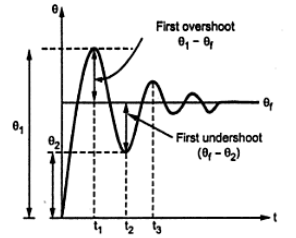
\includegraphics[scale=0.75]{transiente}
    \label{fig:transiente}
\end{figure}

A figura \ref{fig:transiente} mostra um exemplo de transiente que ocorre durante a inicialização do sistema. Durante o projeto de um conversor, é desejado reduzir ao máximo o \textit{overshoot}, bem como o tempo de estabilização do sistema.

\section{Controlador em malha aberta}
Para reduzir o erro fixo na tensão de saída, pode-se utilizar um controlador em malha aberta (\textit{open loop}), de modo a ajustar a tensão até o ponto necessário. A principal desvantagem desse tipo de controle é que ele não reduz os efeitos dos transientes, sendo necessário um ajuste manual da tensão de saída para cara modificação na carga ou na tensão de entrada.

\begin{figure}[H]
    \centering
    \caption{Sistema com controle em malha aberta.}
    \includegraphics[scale=0.75]{openloop}
    \label{fig:openloop}
\end{figure}

A figura \ref{fig:openloop} mostra o diagrama de blocos para um sistema em malha aberta, onde a referência é dada manualmente, podendo ser com o auxílio de um potenciômetro. Nesse trabalho o controlador utilizado foi o CI 3524.
